% Defence slide 3, panel 3: truncate the grown bond back to an affordable chi.
% The bounding box and the chain height match tn_apply.tex exactly, so the two
% panels line up when placed side by side on the slide.
\documentclass[tikz,border=3pt]{standalone}
\usepackage{amsmath,amssymb}
\usetikzlibrary{arrows.meta}
\definecolor{tnbulk}{RGB}{86,196,229}
\definecolor{ink}{RGB}{35,44,58}
\begin{document}
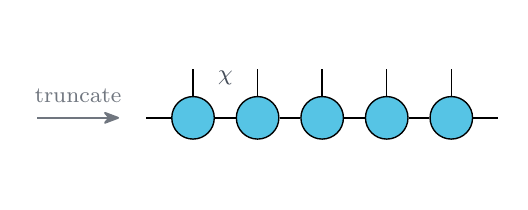
\begin{tikzpicture}[
    W/.style={circle, draw=black, fill=tnbulk, line width=0.5pt,
              minimum size=5.4mm, inner sep=0pt},
    leg/.style={draw=black, line width=0.5pt},
    lab/.style={font=\footnotesize, color=ink!85},
    tag/.style={font=\footnotesize, color=ink!65}]
  \useasboundingbox (-0.10,-0.34) rectangle (5.90,1.62);
  \def\dx{0.82}
  \def\yc{0.475}        % same chain height as the merged chain in tn_apply.tex
  \draw[-{Stealth[round,length=2.4mm]}, color=ink!65, line width=0.7pt]
    (0.02,\yc) -- (1.06,\yc) node[midway, above=2pt, tag] {truncate};
  \foreach \i in {0,...,4} { \node[W] (t\i) at ({2.00+\i*\dx},\yc) {}; }
  \foreach \i/\j in {0/1,1/2,2/3,3/4} { \draw[leg] (t\i.east) -- (t\j.west); }
  \draw[leg] (t0.west) -- ++(-0.32,0);  \draw[leg] (t4.east) -- ++(0.32,0);
  \foreach \i in {0,...,4} { \draw[leg] (t\i.north) -- ++(0,0.34); }
  \node[lab, anchor=south] at ({2.00+0.5*\dx},{\yc+0.30}) {$\chi$};
\end{tikzpicture}
\end{document}
